\begin{pastexam}[label={px:nsysu-115-osds-04}]{中山資工所甲組 115 學年度 第 8 題}
（問答；10 分）

Consider the adjacency matrix of an undirected graph as follows:
\begin{center}
\begin{tabular}{|c|c|c|c|c|c|c|}
\hline
  & A & B & C & D & E & F \\ \hline
A & 0 & 2 & 4 & 0 & 5 & 0 \\ \hline
B & 2 & 0 & 1 & 9 & 0 & 7 \\ \hline
C & 4 & 1 & 0 & 0 & 6 & 10 \\ \hline
D & 0 & 9 & 0 & 0 & 0 & 8 \\ \hline
E & 5 & 0 & 6 & 0 & 0 & 3 \\ \hline
F & 0 & 7 & 10 & 8 & 3 & 0 \\ \hline
\end{tabular}
\end{center}
\begin{enumerate}[label=(\alph*)]
\item (8\%) Starting from vertex A, show the order in which the edges are added into the minimum
spanning tree using Prim's algorithm. Use the weight to represent edges in your answer.
\item (2\%) Let $V$ and $E$ denote the number of vertices and edges in a graph, respectively. What
is the time complexity of Prim's algorithm when it is implemented using an adjacency list and a
binary heap?
\end{enumerate}
\end{pastexam}

\begin{pastsoln}
\textbf{(a)} 依序加入的邊是 $2, 1, 5, 3, 8$（總權重 $19$）。

矩陣裡 $0$ 表示沒有邊（對角線之外）。 矩陣是對稱的，所以是無向圖，邊有 $10$ 條：A--B 2、A--C 4、
A--E 5、B--C 1、B--D 9、B--F 7、C--E 6、C--F 10、D--F 8、E--F 3。 權重都不同，最小生成樹唯一
（資結書定理~24.4）。
\begin{center}
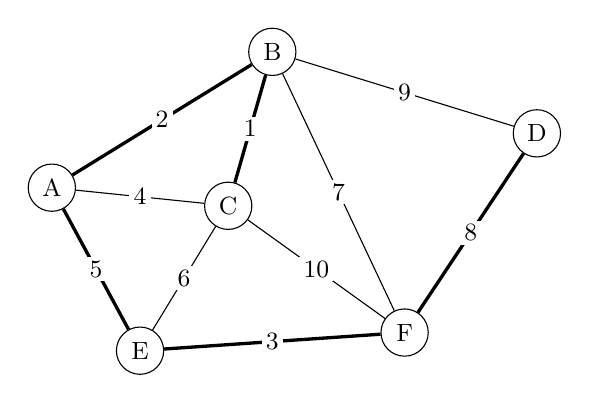
\begin{tikzpicture}[x=1.4cm,y=1.15cm,v/.style={circle,draw,minimum size=6mm,inner sep=0pt,font=\small},w/.style={fill=white,inner sep=1.5pt,font=\small}]
\node[v] (A) at (0,0) {A};
\node[v] (B) at (2,1.5) {B};
\node[v] (C) at (1.6,-0.2) {C};
\node[v] (E) at (0.8,-1.8) {E};
\node[v] (F) at (3.2,-1.6) {F};
\node[v] (D) at (4.4,0.6) {D};
\draw[very thick] (A)--node[w]{2}(B);
\draw (A)--node[w]{4}(C);
\draw[very thick] (A)--node[w]{5}(E);
\draw[very thick] (B)--node[w]{1}(C);
\draw (B)--node[w]{9}(D);
\draw (B)--node[w]{7}(F);
\draw (C)--node[w]{6}(E);
\draw (C)--node[w]{10}(F);
\draw[very thick] (D)--node[w]{8}(F);
\draw[very thick] (E)--node[w]{3}(F);
\end{tikzpicture}
\end{center}
（粗線是最後得到的最小生成樹。）

Prim 演算法（資結書第~24.3~節）：從 A 開始，每一步在「一端在樹裡、一端不在」的邊裡取最輕的，把
另一端加進樹。 每一列列出當時所有的跨越邊：
\begin{center}
\small
\begin{tabular}{clll}
\toprule
步 & 樹裡的頂點 & 跨越邊（權重） & 加入 \\
\midrule
1 & A & A--B 2, A--C 4, A--E 5 & A--B（2） \\
2 & A, B & A--C 4, A--E 5, B--C 1, B--D 9, B--F 7 & B--C（1） \\
3 & A, B, C & A--E 5, B--D 9, B--F 7, C--E 6, C--F 10 & A--E（5） \\
4 & A, B, C, E & B--D 9, B--F 7, C--F 10, E--F 3 & E--F（3） \\
5 & A, B, C, E, F & B--D 9, D--F 8 & D--F（8） \\
\bottomrule
\end{tabular}
\end{center}
加入順序用權重表示是 $2, 1, 5, 3, 8$。 注意第 2 步加的是 $1$，比第 1 步的 $2$ 輕：Prim 每一步只在
跨越邊裡挑，B--C 要等 B 進了樹才變成跨越邊。 （Kruskal 的順序會是 $1, 2, 3, 5, 8$，同一棵樹，順序
不同。）

\textbf{(b)} $O(E \log V)$。

用二元最小堆積存每個不在樹裡的頂點的 key（資結書虛擬碼~24.3）：建堆 $O(V)$；取出最小 $V$ 次，每次
$O(\log V)$；每條邊在兩端各被看一次，最多造成一次降低 key，每次 $O(\log V)$，共 $O(E \log V)$。 總共
$O((V + E)\log V)$，圖連通時 $E \ge V - 1$，寫成 $O(E \log V)$。 （不用帶索引的堆積、改成允許同一個
頂點重複放進堆積的寫法，堆積裡最多 $O(E)$ 個項目，時間 $O(E \log E) = O(E \log V)$，同一級。）
\end{pastsoln}
